\documentclass[11pt,a4paper]{article}
\usepackage{latexsym}
\usepackage{graphicx}
\usepackage{amssymb,amsmath}
\usepackage{mathtools,braket}
\usepackage[english]{babel}
\usepackage{caption}
\usepackage{subcaption}
\usepackage{graphicx}

% Parametri di stampa
\setlength{\topmargin}{-2.5cm} \setlength{\oddsidemargin}{0.3cm}
\setlength{\evensidemargin}{0.3cm}
%
\textheight=23.0truecm \textwidth=16.0truecm
%
\headheight=1.0cm \headsep=1.0cm
%
\renewcommand{\baselinestretch}{1.1}
\setlength{\unitlength}{1mm}

\parindent=6pt

%%%%%%%%%%%%%%%%%%%%%%%%%%%%%%%%%%%%%%%%%%%%%%%%%%%%%%%%%%%%%%%%%%%%%%%%%%%%

\newcommand{\be}{\begin{equation}}
\newcommand{\ee}{\end{equation}}
\newcommand{\bea}{\begin{eqnarray}}
\newcommand{\eea}{\end{eqnarray}}

\newcommand{\op}[1]{\hat {#1}}

%%%%%%%%%%%%%%%%%%%%%%%%%%%%%%%%%%%%%%%%%%%%%%%%%%%%%%%%%%%%%%%%%%%%%%%%%%%%

\begin{document}

%%%%%%%%%%%%%%%%%%%%%%%%%%%%%%%%%%%%%%%%%%%%%%%%%%%%%%%%%%%%%%%%%%%%%%%%%%%%


\section*{Supplementary material}

We report the results of the excitation landscape for the $C_{60}$ and the Aflatoxin molecules. This analysis allows us to investigate the multi-threshold structure for systems with larger number of atoms and/or lower degrees of symmetry respect to the ones presented in the main text. The plots of Fig. \ref{exc-land} evidence that, in both the cases, the sector of localized excitations is very rich and extends well above the first ionization potential of the molecule. These results provide a further confirmation of the behavior already observed in the Table I. 

The growth of the localized sector with the number of atoms of the molecule seems to be a general feature. It can simply explained by observing that bigger molecules behave as wider potential wells and possess a high number of localized Kohn-Sham (KS) orbitals that span a wide energy range. In a simplified two-levels picture, in which $\op V'=0$, the KS empty orbitals $\psi_a$ coincide with the excitation modes defined in eq. (17) and the associated energy is parametrized as $\Omega_a=\epsilon_a-\epsilon_p$. In this case to the increase of the energy range spanned by the localized orbitals it directly corresponds a richer sector of localized excitations.
When $\op V'$ is switched on the excitation modes are expressed as a combination of KS orbitals but the presence of a high number of localized orbitals allows for a rich sector of localized excitations, as confirmed by the results of Fig. \ref{exc-land}.  

\begin{figure}[h]
    \centering
    \begin{subfigure}[t]{0.48\textwidth}
        \centering
        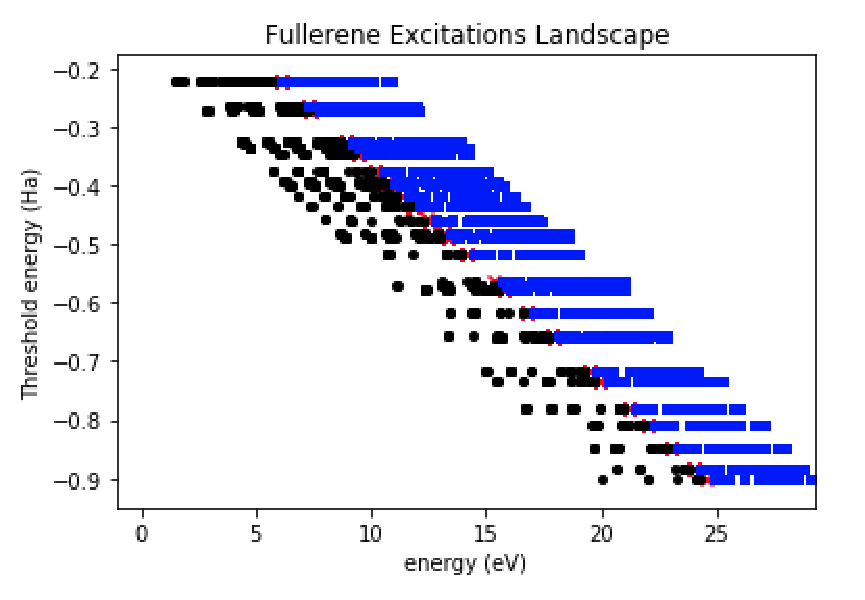
\includegraphics[width=\linewidth]{C60_ExcitationLandscape.eps} 
        \caption{$C_{60}$} \label{fig:b}
    \end{subfigure}
    \hfill
    \begin{subfigure}[t]{0.48\textwidth}
        \centering
        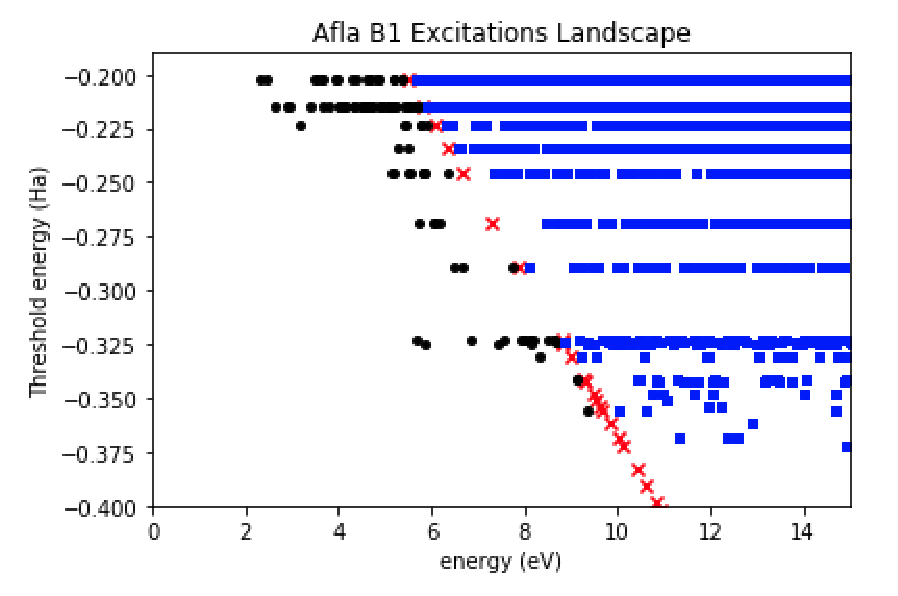
\includegraphics[width=\linewidth]{Aflatoxin_ExcitationLandscape.eps} 
        \caption{Aflatoxin} \label{fig:a}
    \end{subfigure}
    \caption{Excitation landscape for the $C_{60}$ (panel a) and the Aflatoxin (panel b) molecules computed accordingly to the procedure described  in the appendix C. Black circles represent the localized sector and blue squares describe the pseudo-continuum one. }
\label{exc-land}
\end{figure}

%%%%%%%%%%%%%%%%%%%%%%%%%%%%%%%%%%%%%%%%%%%%%%%%%%%%%%%%%%%%%%%%%%%%%%%%%%%%

\end{document}

%%%%%%%%%%%%%%%%%%%%%%%%%%%%%%%%%%%%%%%%%%%%%%%%%%%%%%%%%%%%%%%%%%%%%%%%%%%%
